
\chapter{Introduction}

\section{Fundamentals and neurophysiology of the brain}

The central nervous system (CNS) is responsible for processing information received from all parts of the body. The two main organs of the CNS are the brain and the spinal cord and are entirely composed of two kinds of specialized cells: neurons and glia. The brain is the most complex part of the human body and exerts a centralized control over the other organs. Neurons, the basic working units of the brain, are designed to transmit information within the brain to other nerve cells and to communicate with muscles and gland cells. The complex architecture of the brain is built on the extensive number of interconnected neurons sharing information through specialized connections called synapses. This connection allows  neurons to communicate through an electrical or chemical signals, producing ionic currents that generate electric and magnetic fields. 

The CNS is organized in multiple levels, from simple connections between cells to coordinated cell populations, building a complex architecture of interconnected brain regions. The neural processes at this last level are produced by the dynamic coordination of smaller elements. In the cerebral cortex, all this brain activity is summated and its electric and magnetic fields can be measured on the scalp surface. 

\subsection{Brain anatomy and functions} % http://science.sciencemag.org/content/342/6158/1238411
From an anatomical point of view, the brain can be divided into three parts: the cerebrum, cerebellum and brainstem (Figure \ref{fig:anatomy} a). The cerebrum is the most developed part of the human brain and is divided into the left and right hemispheres. The cerebral cortex consists of the outer layers of the cerebrum and is commonly divided into three parts: the archicortex and the paleocortex, which are the cortical parts of the limbic system; and the outermost layer called neocortex, which is part of the mammalian brain and is involved in higher-order functions. Most of the actual information processing in the brain takes place in the cerebral cortex. In humans, as in mammalian and primates, this structure is folded and results into a much greater surface area in the confined volume of the skull. Folds or ridges in the cortex are referred as gyri, and grooves or fissures are called sulci. The main sulci define four lobes in each hemisphere: the frontal, temporal, parietal and occipital lobes. 

\begin{figure}[ht]
\centering
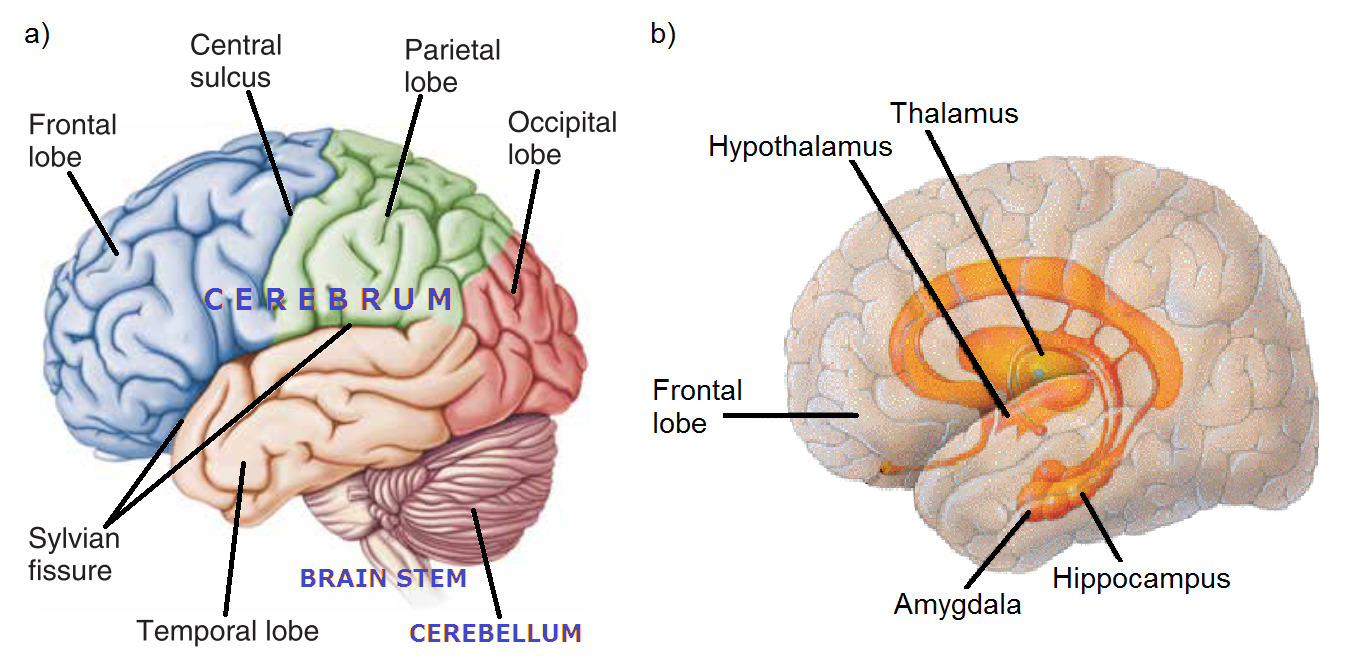
\includegraphics[width=0.9\textwidth]{Images/brainParts.png}
\caption{a) Diagrammatic representation of the major parts of the brain. b) Main structures of the limbic system. Image adapted from \citet{Bear2016}}
\label{fig:anatomy}
\end{figure}

The largest brain lobes, the frontal lobes, are located at the front of each cerebral hemisphere. They are involved in several functions of the body: motor functions, planning, reasoning, impulse control, memory, and language. Behind these, the parietal lobe are located. Their main functions are the processing of sensory information, understanding spatial orientation and body awareness. The temporal lobes play an important role in organizing sensory input, auditory perception, language and speech production, facial recognition, and memory association and formation. The occipital lobes are located at the posterior region of the cerebral cortex. Their main function include visual perception, color recognition, reading comprehension, depth perception and recognition of object movement. 

Below the cortex and on top of the brainstem, a set of structures known as the limbic system (Figure \ref{fig:anatomy} b) are found. These are one of the most primitive parts of the human brain and are involved in the emotions and motivations related to survival. The hippocampus consists of two "horns" that are associated to various processes of cognition related to spatial memory and learning. At its lower end, the amygdalas are located. These are two almond-shaped structures that work as an integrative center for emotions, emotional behavior, and motivation. The thalamus has the important role of relaying sensory input to the cerebral cortex, and also regulates consciousness, and alertness. The hypothalamus, located below the thalamus, is involved in homeostasis processes, controls body temperature, hunger, fatigue, sleep, and circadian rhythms \citep{Purves2001}.

The concept of limbic system has survived to modern times. However, the idea of a unified limbic system is outdated, and the structures and processes related to memory and emotions are more complex, involving also non-limbic areas of the brain \citep{Rolls2015}. In addition,  functions associated with cognition and reasoning require the action of the hippocampus, highly linked to memory processes.

\subsection{The neuronal activity}

Neurons are the basic units of information processing of the nervous system. The brain contains between 50 and 100 billion ($10^{11}$) of neurons \citep{Andreassi2007}, specialized cells whose main function is to receive stimuli and send responses through impulses. Although there are various type of neurons, all of them contain four distinct regions: the cell body or soma, the dendrites, the axon and the axon terminals (Figure \ref{fig:neuron}). 

\begin{figure}[ht]
\centering
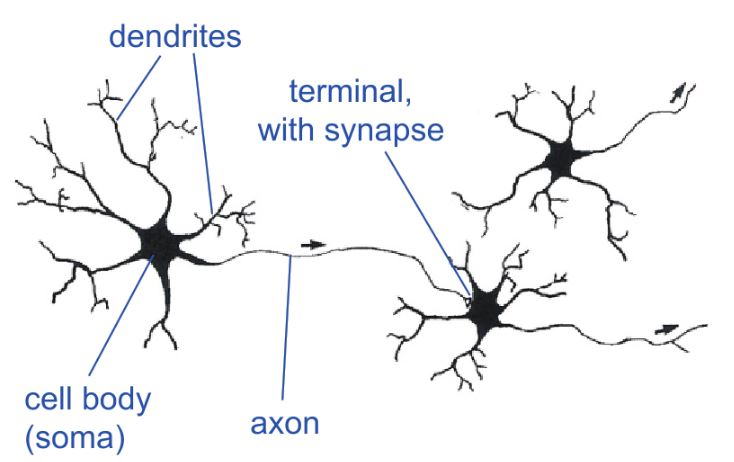
\includegraphics[width=0.65\textwidth]{Images/Neuron.JPG}
\caption{Morphology of the neuron. Image from \citet{Carpenter2012}}
\label{fig:neuron}
\end{figure}


The nucleus is found inside of the soma and is responsible for the synthesis of most of the neuronal proteins and membranes. Axons are specialized in the conduction of action potentials, a particular type of electric impulses, outward from the soma towards the axon terminals. These are small branches of the axon that form the synapses, which are the connections with other neurons, glial cells or muscle fibers. Dendrites are responsible of receiving chemical signals from the axon terminals of other neurons, converting these into electric impulses and transmitting them to the soma. The neurons of the brain have extremely long dendrites with complex branches allowing them to form synapses from a large number of neurons, up to a thousand \citep{Lodish2000}. 


To achieve a long-distance and rapid communication, neurons have special abilities for sending electrical signals along axons. Generally, the information is transmitted in one direction: a presynaptic cell (or sending cell) sends a signal that is picked by the postsynaptic cell (or receiving cell), which can be a dendrite of another neuron, a muscle or a gland cell. The axon terminal of the presynaptic cell contain vesicles filled with neurotransmitters. When a synapsis occurs, these are released to a space called synaptic cleft and they bind with specific receptors located at the plasma membrane of the postynaptic cell (Figure \ref{fig:synapsis})


\begin{figure}[ht]
\centering
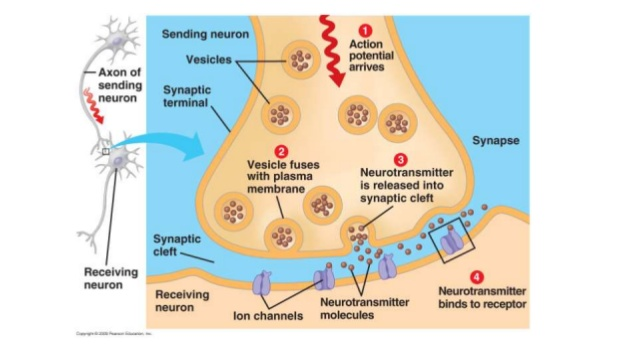
\includegraphics[width=1\textwidth]{Images/synapsis.jpg}
\caption{Communication at a chemical synapse. Image from \citet{Campbell2013}}
\label{fig:synapsis}
\end{figure}

In its resting state, neurons have a negative concentration gradient. This state is called resting membrane potential and is produced by a difference between the number of positive ions outside and inside the neuron. During the resting membrane potential, there are more sodium ions ($Na^+$) outside than inside the neuron and more potassium ions ($K^+$) inside than outside. The number of positive charges outside the neuron is higher than inside, resulting in a negative charge with respect to the exterior of the cell with a typical value of around -70mV. The ions try to balance their concentrations through the flow of ions in and out the cell, but the cell maintains this potential stable through the sodium-potassium pump, forcing potassium back into the cell and pushing sodium out of the cell at the same time. 

The neurons feature different kinds of sodium and potassium channels: the voltage-gated channels that open and close when the membrane potential changes, the ligand-gated channels that open when a neurotransmitter latches onto its receptor, and  mechanically-gated channels that open in response to the physical stretching of the membrane. When stimulus occur or neurotransmitters arrive at the neuron dendrites, the mechanically-gated or ligand-gated sodium channels open and sodium starts diffusing inside the cell, producing a positive increment on the membrane potential. If this potential exceeds the threshold potential, around -55 mV, the large number of voltage-gated sodium channels open rapidly increasing the number of sodium ions inside and depolarizing the cell, triggering the start of the action potential. When the membrane potential reaches around +40 mV, the sodium channels close and the potassium voltage-gated channels open, allowing the diffusion of this substance outside the cell and repolarizing the neuron. In this stage, the diffusion of potassium produces a higher negative membrane potential than in the resting state. This effect is known as hyperpolarization or undershoot, where the membrane potential reaches -75 mV. At this point, potassium gates close and the sodium-potassium pump restores the membrane into the resting potential. Before a new action potential can produced, a refractory period caused by the inactivation of the sodium channels preventing the cell to fire during a period of time. Figure \ref{fig:actionpotential} describe the different phases of the generation of an action potential in a neuron. 

\begin{figure}[ht]
\centering
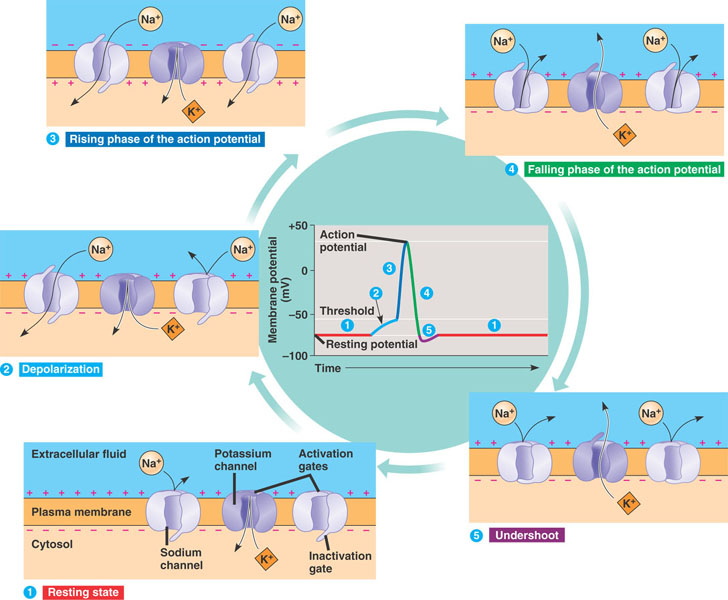
\includegraphics[width=0.95\textwidth]{Images/actionpotential.jpg}
\caption{Generation of an action potential. Image from \citet{Campbell2013}}
\label{fig:actionpotential}
\end{figure}

An action potential only occurs in a limited area of the cell membrane, but the changes in membrane potentials are enough to initiate another action potential in a neighboring space, giving rise to another action potential further down the axon. The refractory period ensures that the information travels only in one direction. When the electric impulse arrive to the axon terminal, neurotransmitters are released, starting the process again in a new neuron. 

Synaptic activity is often the most important source of extracellular current flow \citep{Buzsaki2012} but currents in the brain can also emerge from other non-synaptic sources that do play significant roles in the nervous system \citep{Jefferys1995}. Neuronal activity in the brain gives rise to transmembrane currents that can be measured in the extracellular medium. All neuron types contribute to these currents, but their contribution depends on the shape of the cell \citep{Jefferys1995}. Pyramidal neurons are the most populous kind of excitatory neurons ($2/3$ of the mammalian brain). Most of them are radially oriented in the cortex and orthogonal to the brain surface. Its long dendrites can generate strong dipoles along its axis (see figure \ref{fig:pyramidcell}). 

\begin{figure}[ht]
\centering
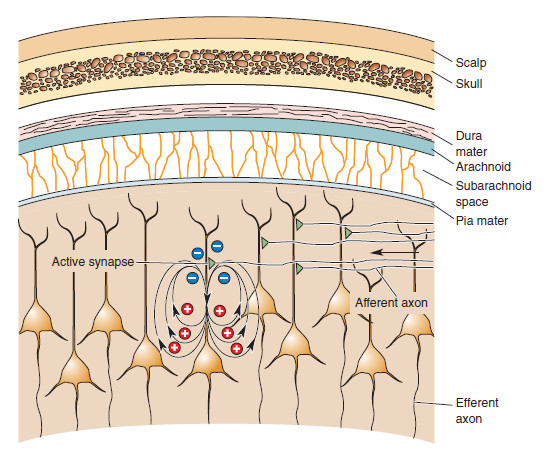
\includegraphics[width=0.75\textwidth]{Images/pyramidcell_dipole.jpg}
\caption{Generation of electrical and magnetic fields by synaptic currents in pyramidal cells. Image adapted from \citet{Bear2016}}
\label{fig:pyramidcell}
\end{figure}

The orientation of this type of cells give rise to an open field, as the dendrites face one direction and the soma another and there is considerable spatial separation between them \citep{Buzsaki2012}. When a group of cells is excited simultaneously, the tiny synchronized signals sum up to generate one larger signal that can be measured on the surface of the head \citep{Bear2016}. The different modalities for measuring the neural activity will be discussed in section \ref{section:EEGMEG}. By contrast, spherically symmetric neurons that whose equal-sized dendrites emerge in all directions, may generate a closed electrical field when several dendrites are simultaneously activated and their potential cancel between each other. In practice, this is rarely the case and the depolarization of a single dendrite generates a small dipole. For this reason, some deep structures can generate dipoles that contribute to the global signal measurable at the extracellular medium \citep{Attal2007}. 

% \subsection{Neural oscillations}

% The synchronized activity of the brain can generate rhythms from low frequencies (0.05 Hz) to high frequencies (600Hz) \citep{Bear2016Neuroscience:Brain} or even to very high frequencies (2500Hz), as reported in recent studies \citep{Usui2015SignificanceEpilepsy}. The classical rhythms described by literature are categorized by their frequency range. \textit{Delta waves} are the slowest, with less than 4Hz and associated to deep sleep. \textit{Theta waves} comprise the interval between 4-7Hz, they appear in both sleeping and awaking states and are extensively linked to the memory function. \textit{Alpha waves}, in the frequency range of 8-13Hz, are associated to quiet, waking states. Conversely, \textit{Beta waves} are associated with active and busy thinking and they comprise the range of 15-30Hz.    
 
	\section{Acquisition systems} 
    \label{section:EEGMEG}
    The summation of the spontaneous brain activity can be measured using different techniques that can be classified into invasive or noninvasive procedures. Noninvasive techniques measure the activity from the scalp. Electroencephalography (EEG) measures the electrical activity using electrodes in contact with the skin and magnetoencephalography (MEG) measures the magnetic activity using gradiometers and magnetometers. Invasive techniques, on the other hand, can measure the activity directly from the cerebral cortex (electrocorticography) or even in deep structures (intracranial electroencephalography). Several biomedical signal processing methods have been used to evaluate and diagnose brain disorders in the time and frequency domains \citep{Sornmo2005} using the information provided by invasive and noninvasive techniques. Due to their small signal-to-noise ratio, specially in noninvasive recordings, the preprocessing of the signals in order to remove artifacts and interferences is essential. This section describes, firstly, the fundamentals of MEG and EEG; and secondly, the differences between the different acquisition modalities.
    
      \subsection{Bioelectric and biomagnetic signals}
As explained before, a group of synchronized neurons can generate an electrical and magnetic field that, depending on the number of involved neurons and the distance between them and the sensors, can provide information about the mechanisms of the brain function. 
        
Brain spontaneous signals are commonly subdivided into different frequency bands, with different properties and functional significance \citep{Huang2016}. These bands are delta (1 to 4 Hz), theta (4 to 8 Hz), alpha (8 to 12 Hz), beta (12 to 30 Hz) and gamma (greater than 30 Hz). Apart from the normal resting-state brain rythms, these techniques can also record other type of time-locked physiological and pathological activity. Event-related potentials (ERPs) are significant voltage fluctuations resulting from evoked neural activity iniciated by an external or internal stimulus \citep{Coles1996}. They are commonly used to analyze sensory and cognitive tasks. 
        
Moreover, some neurological pathologies present electrical characteristics that are observable in the signals. Epileptic seizures present themselves as brief episodes of abnormal synchronous neural activity of the brain \citep{Fisher2005} that can be recorded using EEG and MEG techniques. The epileptic brain also shows other type of time-locked activity during the non-seizure state, called interictal state \citep{Smith2005}. These types of fluctuations are also useful to diagnose, classify and characterize epileptic disorders. Other neurological diseases such as dementias, psychiatric disorders, neurological infections, or encephalopathies also present characteristic features in the measurable brain signals \citep{Smith2005}.
        
        Traditionally, the spectral study of brain signals has been limited to the standard frequency bands (typically up to 50 Hz). However, during the last decades, higher frequency bands of activity have been studied in the normal mammal brain \citep{Buzsaki1992} and also in the pathological brain \citep{Fisher1992}. This was possible due to the technological improvement of the acquisition systems and the computers used for analysis. Among the higher frequency activity, the oscillations commonly known as high frequency oscillations (HFOs) have become an important field of study in epilepsy. HFOs are subdivided into two bands: the ripple band (80 to 200 Hz) and the fast ripple band (200 to 500 Hz) \citep{Gotman2010}, and are considered a promising biomarker of epilepsy, useful to localize the epileptic focus \citep{Jacobs2012}.  
    %hacer una figura de los tipos de señales que mencione    
          \subsection{Electroencephalography}
          %kamarajan
          EEG signals (usually called simply EEG) were recorded on the human scalp for the first time in 1924 in by Hans Berger \citep{Sornmo2005}. The EEG evolved during the second part of the $20^{th}$ century and became a tool used to study several neurological diseases. However, with the appearance of computed tomography (CT) and magnetic resonance imaging (MRI), the technique lost strength in the neurologists' community, mainly because its poor spatial resolution \citep{Zifkin2009}. The technological advances of the last decades allowed to record and save larger amounts of EEG data, enhancing the spatial resolution of the technique by adding more electrodes and increasing the signal-to-noise ratio of the signals. Moreover, the improvement of the processing capabilities of computers fastered the development of new signal analysis techniques useful to evaluate and diagnose the normal and pathological brain. 
 
To measure electrical signals outside the head, neural activity must travel from the brain through the meninges, the skull, and the scalp layers before reaching the electrodes. All these layers are electrically are insulating layers with poor conductivity and equivalent to capacitors. In order to improve the conductivity between the scalp and electrodes, conductive gel is commonly used. Even after proper enhancement of the skin-electrode contact, the potentials are very small and must be boosted. For this reason, other important part of the EEG systems, and in general any biomedical signal acquisition system, is the amplifier. Its main function is to maximize the signal-to-noise ratio on the measured voltage and to increase the signal above the noise level that may be introduced in the latter elements \citep{Jackson2014}.

As any electric other signal, the voltage is measured by the electrodes with respect to a  reference point. The most common electrode montages include the bipolar, where the potential difference between a pair of electrodes is measured, and the unipolar, where the potential of an electrode is compared to a neutral electrode or to the average of all electrodes. 

The EEG is commonly recorded using the international 10/20 system \citep{Klem1999}. This montage employs 21 electrodes attached to the surface of the scalp. The positions are determined using two reference points: \textit{nasion}, which is the delve at the top of the nose; and \textit{inion}, which is the bony lump in the mid-line at the back of the head (see Figure \ref{fig:1020EEG}). From these points, the skull perimeters are measured in the transverse and medial planes. The electrode locations are determined dividing this perimeters into 10\% and 20\% intervals. The 10/20 electrode system is still used with clinical and research purposes, but if EEG is to be used for brain imaging, several studies claim that at least 64 electrodes should be used \citep{Gotman1982}. In denser electrode montages, the most common procedure is to extend the standard 10/20 system placing the electrodes every 10\% along the medial-lateral contour and introducing new contours between the existing ones. 

EEG is a popular tool mainly because its low-cost and portability. For this reasons it is used in many clinical applications: to diagnose epilepsy, to assess sleep, to study other neurological disorders, to develop brain computer interface (BCI) applications, or to test the brain response under different conditions and stimuli. The main advantages and disadvantages of EEG will be discussed in the next sections. 

\begin{figure}[ht]
\centering
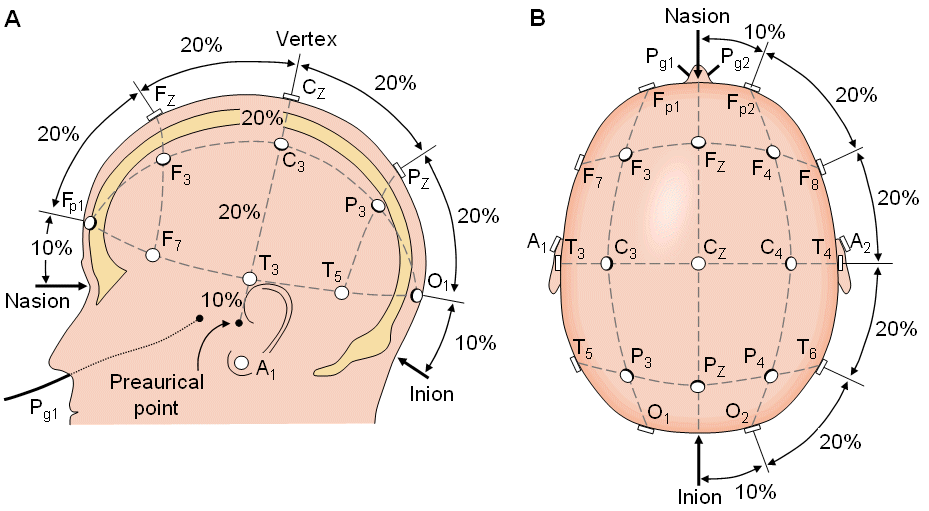
\includegraphics[width=0.95\textwidth]{Images/1020EEGsystem1.png}
\caption{The international 10-20 system seen from (A) left and (B) above the head. A  = Ear lobe, C  = central, Pg = nasopharyngeal, P  = parietal, F  = frontal, Fp = frontal polar, O  = occipital. Image adapted from \citet{American1991}}
\label{fig:1020EEG}
\end{figure}
%añadir alguna referencia mas?
          \subsection{Magnetoencephalography}

Electric currents measured by EEG are necessarily accompanied by electromagnetic fields. The possibility to record the cerebral magnetic field aroused great interest: as conductivity varies essentially only along the head radius from skull to scalp, the magnetic field outside of the head should be unaffected by these tissues above the cortex \citep{Hari2012}. This characteristic of MEG is essential: MEG is a much more expensive technique than EEG. However, the high number of sensors and the non-distortion of the acquired signals greatly improve the spatial resolution, maintaining the millisecond time resolution of EEG. For these reasons, MEG allows real-time tracking of brain activation sequences in the source space. 

The first magnetoencephalographic recording was performed by David Cohen in 1968 \citep{Cohen1968} using copper coils to register the activity. Magnetic fields are considerably lower than electric fields, typical amplitudes of MEG signals are less than 1 pT \citep{Lee2014}. For this reason, these first recordings contained low SNR signals. In 972, Cohen used SQUID sensors (Superconducting Quantum Interference Device) obtaining recordings with increased SNR, comparable to EEG. To preserve its super-conductive properties, these type of sensors have to be maintained at very low temperatures (-269º), immersed in liquid helium \citep{Hari2012}. Currently, MEG systems are composed of 140 to 300 sensors distributed throughout the head. The recordings are performed using a thermally insulated container, known as dewar, where the sensor coils are kept in a helmet that does not touch the patient's head during recordings. 

Figure \ref{fig:MEGdiagram} shows a diagram of the typical parts of a MEG system. To reduce the strong magnetic environmental noise, MEG recordings have to be carried out inside a magnetically shielded room. The participant can be sitting or lying down, as close as possible to the MEG sensors. Typically, the patient's head shape is digitalized to allow an improved coregistration with an individual or standard anatomical MRI \citep{Gross2013}. As the helmet does not touch the patient's head, the position of the head must be known during the recording. To do so, a Head Position Indicator is used which provides information about the position of the MEG system with respect to the head with an accuracy of about 2mm \citep{Hari2004}. During MEG recordings, it is possible to record supplementary signals: the electrooculogram (EOG) and the electrocardiogram (ECG) are highly recommendable to posterior preprocessing of artifacts \citep{Gross2013}. Furthermore, EEG and electromyogram (EMG) can also be recorded simultaneously. 

\begin{figure}[ht]
\centering
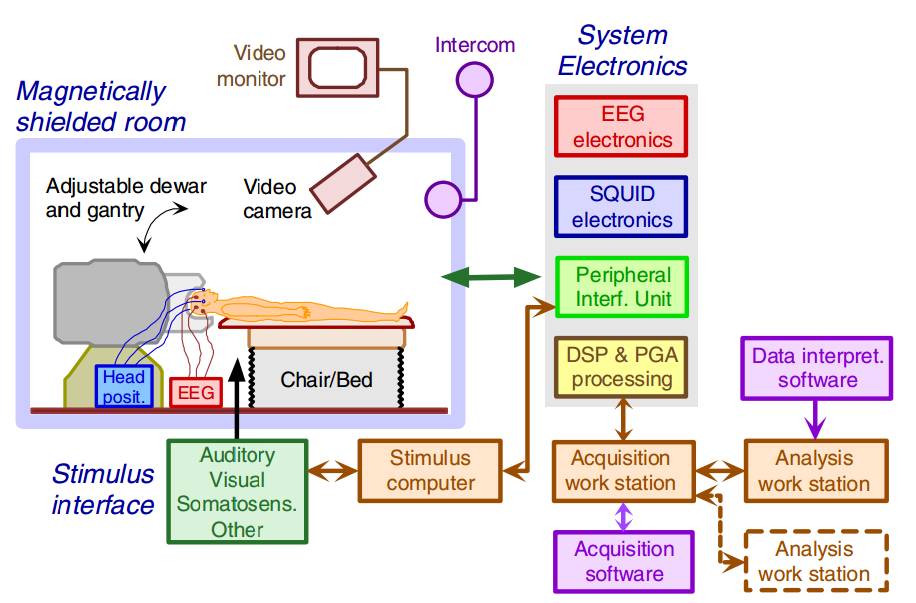
\includegraphics[width=0.85\textwidth]{Images/MEGsystem.png}
\caption{Block diagram of a typical MEG system. Adapted from \citet{Sternickel2006}}
\label{fig:MEGdiagram}
\end{figure}   

A SQUID is a converter from magnetic flux to voltage. Furthermore, to increase the detection efficiency, pickup coils are needed. Among various types of pickup coils, the most common are magnetometers and gradiometers. While magnetometers have better sensitivity to deep and cortical sources, they are more vulnerable to external noises than gradiometers, which in turn are capable of measuring the tangential components of neuroelectric activity. Gradiometers can be axial or planar (see Figure \ref{fig:gradiometers}). Axial gradiometers have higher baseline (distance between the centers of pick-up coils) than planar gradiometers, this provide better sensitivity to deeper sources. For cortical sources, planar gradiometers have better sensitivity to perpendicularly-oriented dipoles. Depending on the thickness of the MSR, the combination of the different type of sensors is selected \citep{Lee2014}. 


\begin{figure}[ht]
\centering
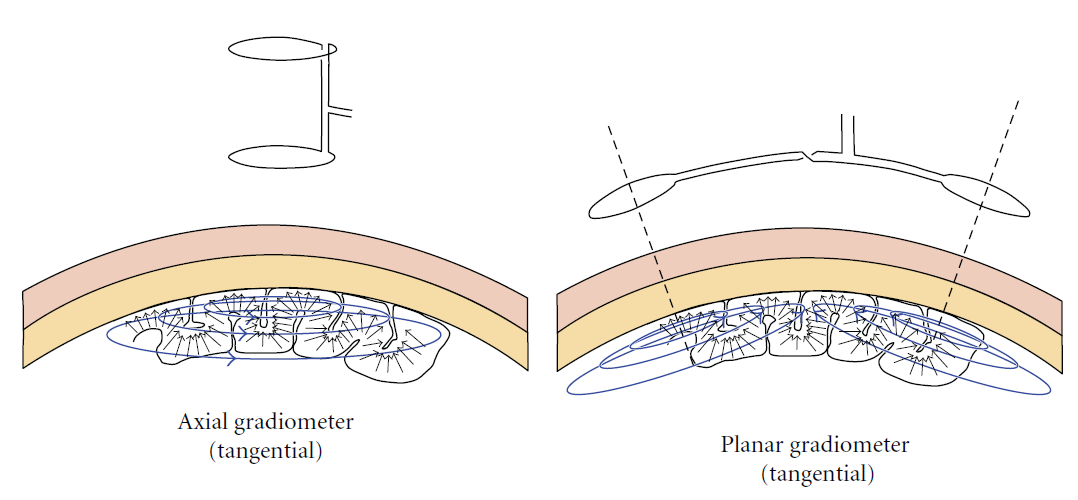
\includegraphics[width=0.85\textwidth]{Images/axialPlanarGradiometer.PNG}
\caption{(Left) MEG setup measuring the tangential components of neuroelectrical activity, using an axial gradiometer. (Right) MEG setup measuring the tangential components of neuroelectric activity, using a planar gradiometer. Image from \citep{Wendel2009}}
\label{fig:gradiometers}
\end{figure}      

Due to the complexity of the measure system, MEG is an expensive technique only available in few laboratories and clinical centers. However, during the recent years, this neuroimaging tool has become more and more important to evaluate brain localized activity at the millisecond scale, providing good spatial resolution. It is important to remark that the spatial resolution in the source space  depends on several factors including number of channels, noise, source depth, source strength, the source model and the inverse modeling method that is used to localize the activity \citep{Harti1988}. Under optimal conditions, in superficial sources the resolution that can be obtained is of few milliliters but this number increases when the sources are deeper. 

          \subsection{Comparison between MEG and other noninvasive neuroimaging methods}
         
MEG noninvasively evaluates the temporal dynamics of neurological processes with a millisecond resolution and with higher spatial resolution than standard EEG. Other techniques, like functional MRI (fMRI) are capable of analyzing the brain function with a spatial resolution of millimeters \citep{Liu2006}. Recently, there is increasing interest in using techniques that combine excellent temporal resolution with those that provide a superior spatial resolution \citep{Liu2015}. For this reason it is important to understand which are the advantages and disadvantages of these techniques and the role of MEG recordings in noninvasive neuroimaging systems. 
          
          \subsubsection*{MEG vs EEG}

EEG and MEG waveforms are similar, as both techniques record the electromagnetic activity generated by the same primary currents in the brain \citep{Niedermeyer2010}. The magnetic field generated by a current dipole in a spherical volume is also dipolar, but the electric and magnetic dipole appear rotated 90 degrees \citep{Hari2004}. Consequently, the sensitivities of both techniques depend on the orientation of the dipoles. MEG gradiometers are more sensitive to tangential sources, while EEG electrodes are more sensitive to deep and radial sources \citep{Hari2004}. Thus, both techniques are considered to provide provide complementary information \citep{Sharon2007}. Several studies have reported the added value of combining MEG and EEG data when performing brain source localization \citep{Aydin2015,Sharon2007}. 


\begin{figure}[ht]
\centering
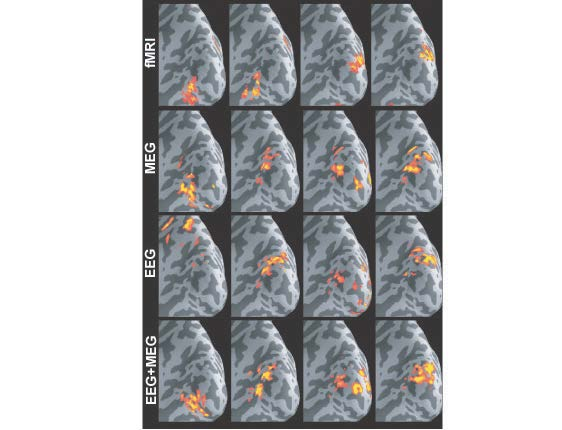
\includegraphics[width=1\textwidth]{Images/eegmegfmri.jpg}
\caption{Spatial response patterns from fMRI and MEG/EEG in focally-stimulated visual cortex. Image from \citet{Sharon2007}}
\label{fig:eegmegfmri}
\end{figure}      

The biggest disadvantage of scalp EEG is its low spatial resolution. The involvement of large areas of brain tissue is required to record EEG \citep{Falco-Walter2017}. Spatial resolution of EEG can be enhanced by increasing the number of sensors. High density EEG (hdEEG) is a recent technique that can record almost 300 channels \citep{Klamer2015}, remarkably enhancing the spatial resolution of the technique. However, the high resistivity of the skull and the more conductive scalp distort and attenuate the electric signals \citep{Cuffin1979}, whereas they do not affect the magnetic fields, conferring a localization advantage of MEG over EEG. Furthermore, the distortion produces the need of more sophisticated forward models \citep{Klamer2015}, and for this reason, MEG recordings are more frequently used in the source space analysis. Other disadvantages of EEG over MEG rely on the sensitivity to movement artifacts, the time of preparation of the subjects, and the need of a reference sensor \citep{Sharon2007} given that MEG provide absolute measures of the magnetic fields. 

The advantages of EEG with respect to MEG are associated with the complexity of MEG systems. The SQUIDs and the magnetically shielded room require a costly set up that has prevented the widespread use of this technique in hospitals and research centers. \citep{Sternickel2006}. However, during the last years, the number of MEG systems has increased notably and new types of MEG sensors, not based in supeconductive materials, are being developed \citep{Boto2017}.  

		\subsubsection*{MRI and fMRI with MEG}
		
Magnetic resonance imaging is the structural imaging modality of choice to screen neurological patients \citep{Assad2015}. This noninvasive technique uses non-ionizing radiation to create useful diagnostic images. The most common MRI procedures include 1.5 or 3 Tesla (T) axial whole brain images with thin slices. The high resolution (sub-milimetrical ) of this technique allows the identification of differences and abnormalities in brain studies. MRI can also be used to create volumetric data of the brain, providing data for accurate surface models of an individual patient's brain \citep{Xu1999}. Volumetric data is commonly used in MEG studies to obtain the regions and extent of the observed scalp data at the source level in cortical and subcortical locations. 
	
The electrodynamic of the brain is accompanied by a series of neurochemical processes that ultimately result in a measurable change in the MR signal. These processes cause combined effects in cerebral blood flow, blood volume, oxygen extraction and metabolism that are local to the site of cerebral activity \citep{Belliveau1991}. This is the basis of fMRI. The transient increase in the MR signal is usually termed the BOLD haemodynamic response function (HRF). When a stimulus is produced, it take several seconds for the HFR to peak and return to baseline \citep{Hall2014}. The latency and longevity of the HFR limit temporal resolution to approximately 5 seconds, much inferior to the millisecond resolution of MEG. Multimodal imaging using MEG and fMRI in parallel offers the possibility of measurement of neurophysiological processes with excellent spatial and temporal resolution. Several recent studies have successfully evaluated different pathological and physiological processes combining both techniques \citep{McWhinney2016,Tewarie2016,Garces2016,Cetin2016}.  

          \subsection{Invasive EEG and MEG} %pensar si es mejor este apartado antes o despues del de other neuroimaging techniques
Brain activity can also be recorded directly on the brain cortex using grid electrodes, or in deep regions using strip electrodes. The first give rise to the so-called Electrocorticography (ECoG), while the second is known as intracranial EEG (iEEG), and both techniques require a surgical procedure to be placed in the head. Due to the high invasiveness of these techniques, electrodes are only implanted in subjects with a pathology that requires precise evaluation at millimetric spatial resolution of target brain regions \citep{Grova2016}, such as refractory epilepsy.

Invasive EEG provides excellent time and spatial resolution within the implanted region. The spatial resolution is improved not only by the proximity of the electrode to the source but also due to the higher signal-to-noise ratio and because signal are not affected by the tissue distortion. Consequently, these techniques are considered the ``gold standard'' for the evaluation of localized brain activity \citep{Santiuste2008}.

However, invasive recordings have some significant drawbacks: risks of morbidity because of invasiveness, high cost, limited availability, limited spatial sampling and the possibility of inaccurate localization \citep{Santiuste2008}. High invasiveness is the main disadvantage of these techniques, preventing the studies in large populations of subjects  and consequently limiting the research to specific kinds of patients. Another important disadvantage of iEEG and ECoG is that the spatial sampling is limited to the area of implantation, making impossible the visualization of the whole-head activity. 

Surgical intervention is one of the most common treatments for pharmacorresistant focal epilepsy \citep{Ramey2013}. MEG, EEG and MRI are the first noninvasive tests in any pre-surgical work-up \citep{Grova2016}, and their role is to help delimitate the area of resection. However, this is not always possible and the implantation of electrodes is needed. In this scenario, noninvasive techniques also play a major role: they are used to delimitate the area where the electrodes should be implanted. Furthermore, there is increasing interest in the simultaneous evaluation of noninvasive MEG and EEG with invasive EEG recordings. While the first can provide a global evaluation of the brain, the second can describe in detail what is happening in deep localized regions \citep{Grova2016}

\section{Source localization of epileptic focus in pharmacoresistant epilepsies}

The most important diagnostic tool in epileptic disorders is performed using invasive and noninvasive electrophysiology. There is a strong historical link between epilepsy and neurophysiology research that has fostered the advance in both fields \citep{Schomer2010}. In this section, the basic clinical characteristics of epileptic disorders are described, especially for refractory epilepsies, which are resistant to pharmacological treatment. After that, the existing signal analysis methods to localize the area generating the seizures are explained.

\subsection{Epilepsy}

Epilepsy is a chronic pathology that affects about 1\% of the world population \citep{Ramey2013}. It is defined by atypical electrical activity in the brain, which often leads to neurobiological, cognitive and psychological consequences. Epilepsy consists of recurrent paroxysmal events called seizures, defined as hyper-synchronized or excessive abnormal activity of the brain \citep{Frohlich2016}.

When a patient suffers more than one seizure, EEG is commonly used to diagnose epilepsy. The purpose of EEG is to look for epileptiform abnormalities, but EEG recordings are rarely performed during an epileptic seizure. Instead, neurologists look into the resting state recordings, also called as interictal recordings. About 50\% of patient show anomalous and distinctive patterns called interictal epileptiform discharges (IEDs) in its first EEG recording \citep{Smith2005}. IEDs are not only used to diagnose epilepsy, but also as biomarkers of epileptic foci. 

Epileptic seizures can be classified using several different schemes. The can be either \emph{idiopathic} (cause unknown) or \emph{symptomatic} (consequence of another disorder of the brain); \emph{partial} (one focal onset zone) or \emph{generalized} (no clear foci); \emph{simple} (no loss of consciousness) and \emph{complex} (loss of consciousness) \citep{Frohlich2016}. Moreover, their classification can be based on the observation of specific neuroelectrical activity and clinical features that enable the definition of \emph{epilepsy syndromes} (Childhood absence epilepsy, Lennox-Gastaut syndrome, benign rolandic epilepsy, etc.) . Finally, the seizures originated at the same areas of the brain usually share some clinical features (semiology) and EEG patterns \citep{Kass2017}. In this sense, seizures can be grouped into \textit{frontal, mesial temporal, lateral temporal, parietal} and \textit{occipital}.

The primary therapy for epilepsy is anti-epileptic drugs (AEDs). Currently, there are more than 20 different AEDs that reduce or eliminate seizures for most patients \citep{Franco2014}. However, around 20 to 40\% of patients with idiopathic generalized epilepsies and up to 60\% of patients with focal epilepsy may manifest resistance to medication \citep{Alexpoulos2013}, experiencing disabling seizures after being treated with three or more different drugs. If the epilepsy is partial, the most promising treatment for these patients is the surgical removal of the epileptogenic zone (EZ), defined as the \textit{the minimum amount of cortex that must be resected (inactivated or completely disconnected) to produce seizure freedom} \citep{Luders2006,Jacobs2012}. To obtain a successful surgical outcome, neurosurgeons have to previously delimit the EZ with accurately and precisely. Invasive and noninvasive electromagnetic recordings play a decisive role in the presurgical evaluation of epileptic refractory epilepsy. 

\subsection{The presurgical evaluation of epilepsy}

Surgery is the only treatment that can possibly cure epilepsy in pharmaco-resistant patients. The aim of epilepsy surgery is to remove the EZ with the preservation of the eloquent areas \citep{Rosenow2001}. During the last years, noninvasive functional neuroimaging techniques have proved to be suitable in the presurgical assessment of epilepsy in the majority of cases. Nevertheless, in some patients (25 to 50\%) the noninvasive localization is not possible and the use of intracranial EEG is required \citep{Pittau2014}. In preoperative evaluation, the site and extent of the epileptic focus is determined in a multimodal assessment. The pre-evaluation often consists of dedicated structural MRI, functional MRI, and interictal and ictal EEG and MEG recordings.

As previously explained, the EZ is a theoretical zone that cannot be spatially defined. However, there are several cortical zones highly linked with the epileptic brain that can be delimited (see Figure \ref{fig:epiZones}). Using structural MRI, the epileptogenic lesion can be determined, if exists. The \emph{functional deficit zone} is the region of the cortex with an abnormal function. It can be determined with neuropsychological testing or fMRI. The \emph{seizure-onset zone (SOZ)}  is the area where the clinical seizures originate. To determine the SOZ, EEG, MEG, or iEEG recordings during the ictal period are required. The \emph{irritative zone} is the area that generates interictal epileptiform discharges (IEDs) in MEG and EEG. During the last few years, the role and the extent of the \emph{HFO zone}, an area that is considered a further piece of information to better circumscribe the EZ \citep{Tamilia2017}.

\begin{figure}[ht]
\centering
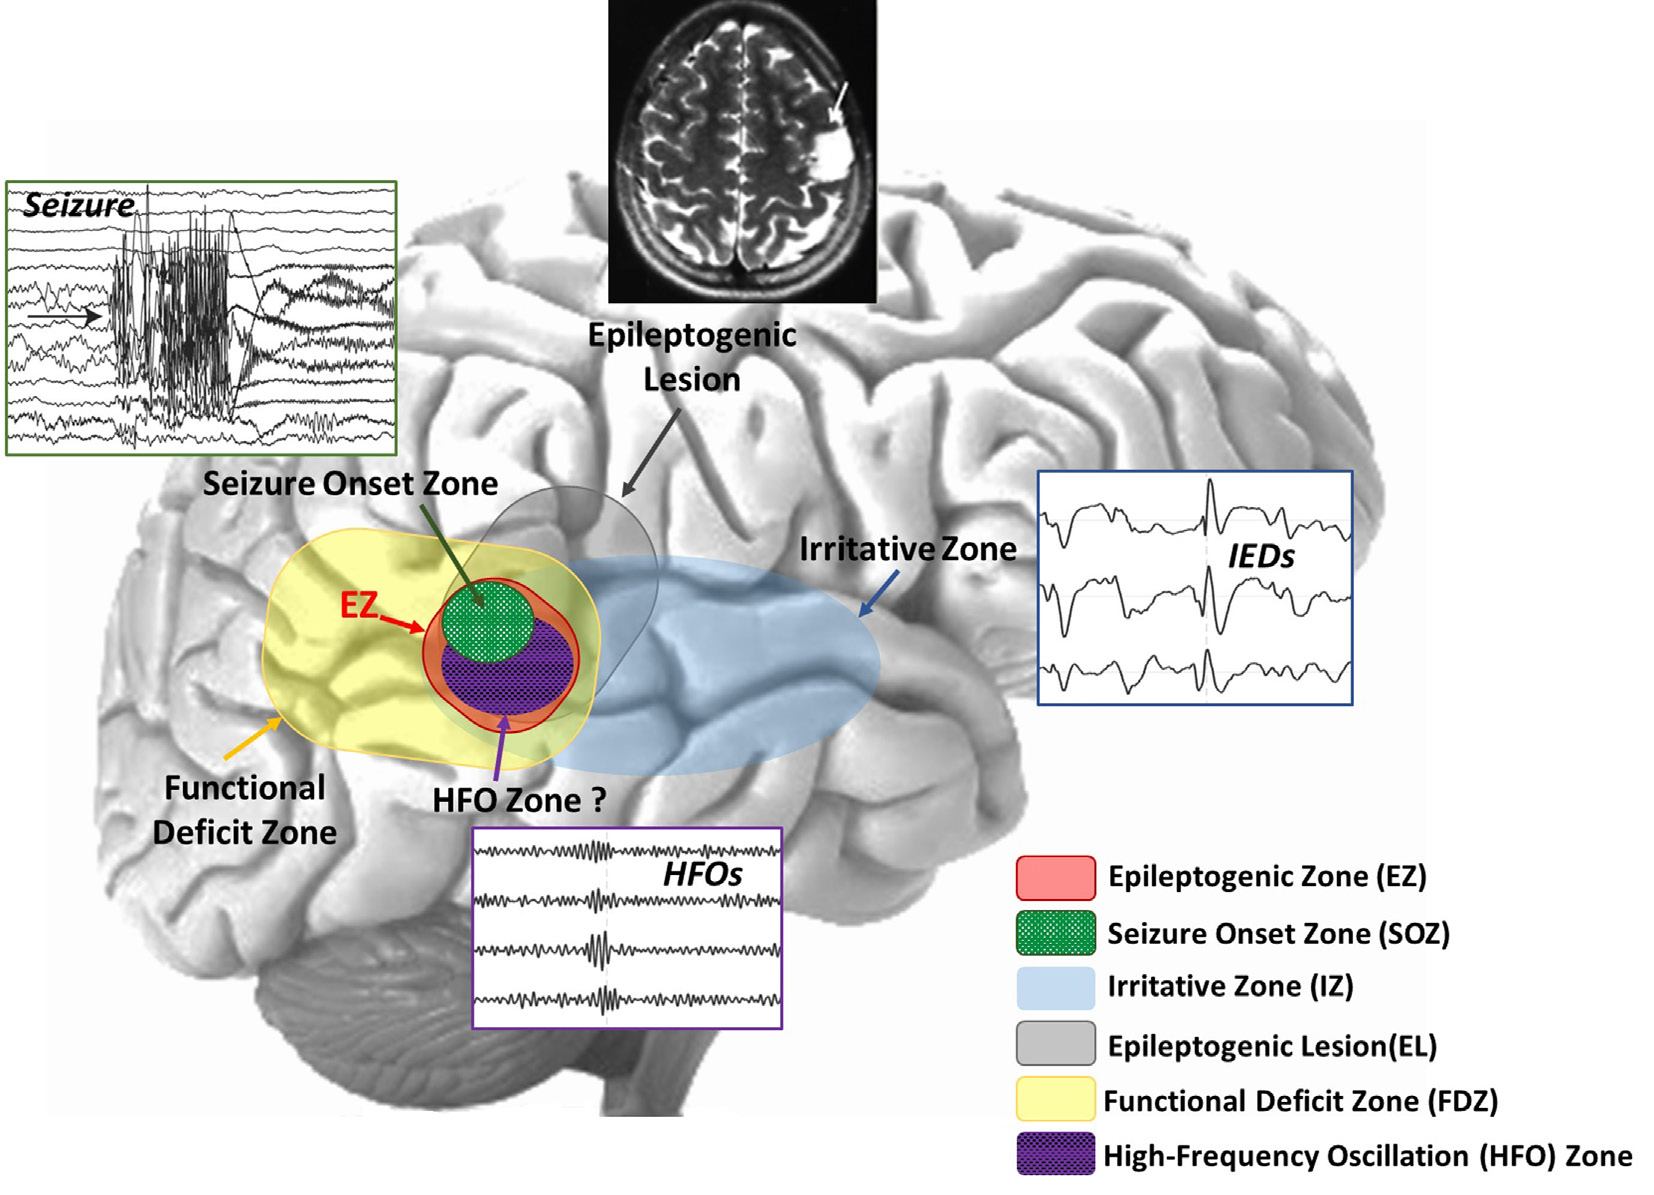
\includegraphics[width=1\textwidth]{Images/epiZones.png}
\caption{Schematic representation of the overlapping cortical zones in epilepsy. Different cortical zones are estimated during the pre-surgical evaluation of a patient with epilepsy. These zones can often overlap, providing the epileptologist with concordant findings for the delineation of the epileptogenic zone (EZ). The high-frequency oscillation (HFO) zone is another potentially epileptogenic area that has been recently added to this picture as a further piece of information to circumscribe the EZ. Image from \citep{Tamilia2017}}
\label{fig:epiZones}
\end{figure}      

The SOZ is generally considered the best estimate of the EZ and is the region removed in most epilepsy surgeries \citep{Luders2006}. \citet{Talairach1973} were the first to assume that the EZ could be defined by placing invasive electrodes in the SOZ and in the regions where the seizure spread \citep{Talairach1966}. This procedure is commonly known as stereoelectroencephalography (SEEG). In addition to the invasiveness of the technique, ictal recordings are needed to determine the SOZ by these means. Clinical seizures are unpredictable and difficult to be captured by EEG. This procedure is costly and requires very long recording times and discomfort for the patient. Sometimes, neurosurgeons anesthetic drugs that can activate the seizure foci within 30 seconds, such as etomidate\citep{Ebrahim1986}.

Even when the monitoring of the SOZ is possible, the entire removal of this region does not always lead to a successful outcome  \citep{Rummel2015}. Studies have shown positive outcomes that can vary between 40\% to 80\% of patients, depending on the type of epilepsy \citep{Schulze2014}. Furthermore, due to the spatial limitation of iEEG, the exact boundaries of the SOZ and the extent of overlap with the EZ remain unknown. 

The inability to localize the SOZ limits the decision making for epilepsy surgery \citep{Berg2003,Uijl2005}. For these reasons, the evaluation of interictal recordings using noninvasive techniques can help in the delimitation of the EZ. Interictal epileptiform events appear more often than seizures and reduce patient discomfort \citep{Staba2014}.

\subsection{Interictal biomarkers for localization of the epileptic focus}

Epileptic seizures are a specific biomarker of epilepsy and the localization of the epileptic focus. However,  their unpredictable nature and irregular rate of occurrence, ictal recordings are not ideal in terms of time, cost, or risk for this purpose \citep{Staba2014}. Other useful transient pathological disturbances can be recorded between the ictal seizures being the most important the interictal epileptiform discharges (IEDs) and the pathological high-frequency oscillations (HFOs) between 80Hz and 600 Hz. 

\subsubsection{Interictal epileptiform discharges}

The neurobiological mechanisms generating IEDs are diverse because focal IEDs show a high variability patterns: spikes, sharp waves, bursts of fast spikes, sequences of fast oscillations, etc., even in the same patient (see Figure \ref{fig:iedtype}). In spite of these high differences, IEDs of pharmacoresistant epilepsy have been well defined \citep{deCurtis2012}. Interictal spikes related to this type of epilepsies are initiated by large post-synaptic depolarizations. It has been demonstrated that spikes that appear near the SOZ are different from the ones produced in remote regions by synchronized activity, suggesting that these events represent an interplay of multiple neuronal types within complex neuronal networks \citep{Keller2010}. 


\begin{figure}[ht]
\centering
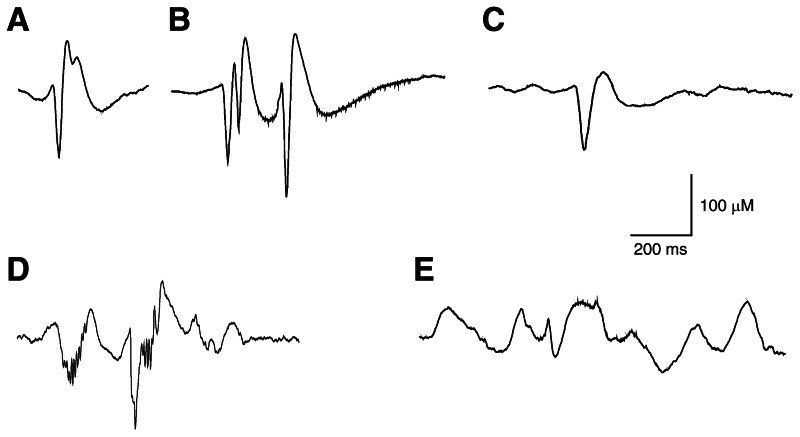
\includegraphics[width=1\textwidth]{Images/decurtisf1.jpg}
\caption{Interictal epileptic discharge (IED) patterns recorded in human partial epilepsies with intracranial electrodes. \emph{a} Interictal spike; \emph{b} group of interictal spikes, \emph{c} sharp wave; \emph{d} fast activity (brushes); \emph{e} paroxysmal slow activity superimposed to slow spikes. Image from \citep{deCurtis2012}}
\label{fig:iedtype}
\end{figure}      

Interictal spikes are characterized by a large-amplitude rapid component lasting from 50 ms to 100 ms and usually followed by a slow wave of 200 ms to 500 ms in duration \citep{Nowak2009}. IEDs can be detected in MEG and EEG recordings. Its sensitivity highly depends on the orientation and deepness of the sources. While several studies have found higher sensitivity in MEG than EEG \citep{Ramantani2006,Zijlmans2002,Iwasaki2003}, other studies claim that the two techniques perform almost the same, achieving higher sensitivity when both are used simultaneously \citep{Baumgartner2004}.

The main disadvantage of using IEDs as a biomarker for the delimitation of the EZ lies in the fact that these are generated is the irritative zone (IZ), an area that only partially overlaps the EZ (see Figure \ref{fig:epiZones}), and can appear distant to the lesional site \citep{Penfield1954}. The relationship between the SOZ (generally more linked with the EZ) and the IZ is still an unresolved issue and an important research topic. For some patients, areas generating high spike rates are highly correlated ($\sim$75\%) with the areas where the seizure initiated. However, in other subjects these areas appear dissociated \citep{Bartolomei2016}. Due to the lack of concordance between these two areas, there is increasing interest in finding other interictal biomarkers to delimitate the EZ. During the last decade, HFOs have emerged as a promising biomarker for epileptogenicity \citep{Jacobs2012}. 

\subsubsection{High-frequency oscillations}

HFOs are defined as spontaneous patterns above the baseline, clearly distinguished from noise and with at least four oscillations \citep{Worrel2012}. They appear in the frequency range of 80 Hz to 500 Hz and are commonly classified into ripples (80 Hz to 200 Hz) and fast ripples (200 Hz to 500 Hz). Several recent studies have evaluated high-frequency oscillations as a specific biomarker for epileptogenicity \citep{Jacobs2012,Fujiwara2012,YanPing2015}.

High-frequency oscillations appear also in the normal mammalian brain, and are then called physiological high-frequency oscillations. However, several studies have pointed out that there could be important differences between the neuronal processes of the pathological and physiological HFOs \citep{Staba2014}. Although the generation of pathological HFOs is still an open question, several observations have shown that these oscillations are generated by the neurons near the epileptogenic focus \citep{Jefferys2012}. There are studies that even suggest that HFOs could have a causal role in the ictogenesis, which would have an impact in improving the epilepsy treatment \citep{Jiruska2010}.

The relation between epileptic spikes and HFOs is still an open discussion. Early studies reported that most of the observed fast ripples appeared at the same time as spikes \citep{Engel2009}. \citet{Urrestarazu2007} defined three different cases in which an HFO can occur: (i) completely independent of IEDs, (ii) together with spike and visible in the unfiltered data and (iii), together with the spike but invisible in the unfiltered spike (Figure \ref{fig:HfoSpike}). Subsequent studies provided evidence that HFOs and spikes have different neurophisiological mechanisims. On the one hand, HFOs seem to be more specific to the SOZ \citep{Jacobs2008,Crepon2010}. On the other hand, when the epileptic medication is reduced, HFOs tend to increase in number while IEDs do not exhibit this trend \citep{Zijlmans2009}. This indicate that both biomarkers behave differently under changing conditions. Furthermore, spikes co-occurring with HFOs have shown to be more closely related to the SOZ \citep{Jacobs2008} than those occurring alone. This differentiation can be helpful to distinguish between \emph{good} and \emph{bad} spikes, originating or not inside the EZ \citep{Tamilia2017}.   


\begin{figure}[ht]
\centering
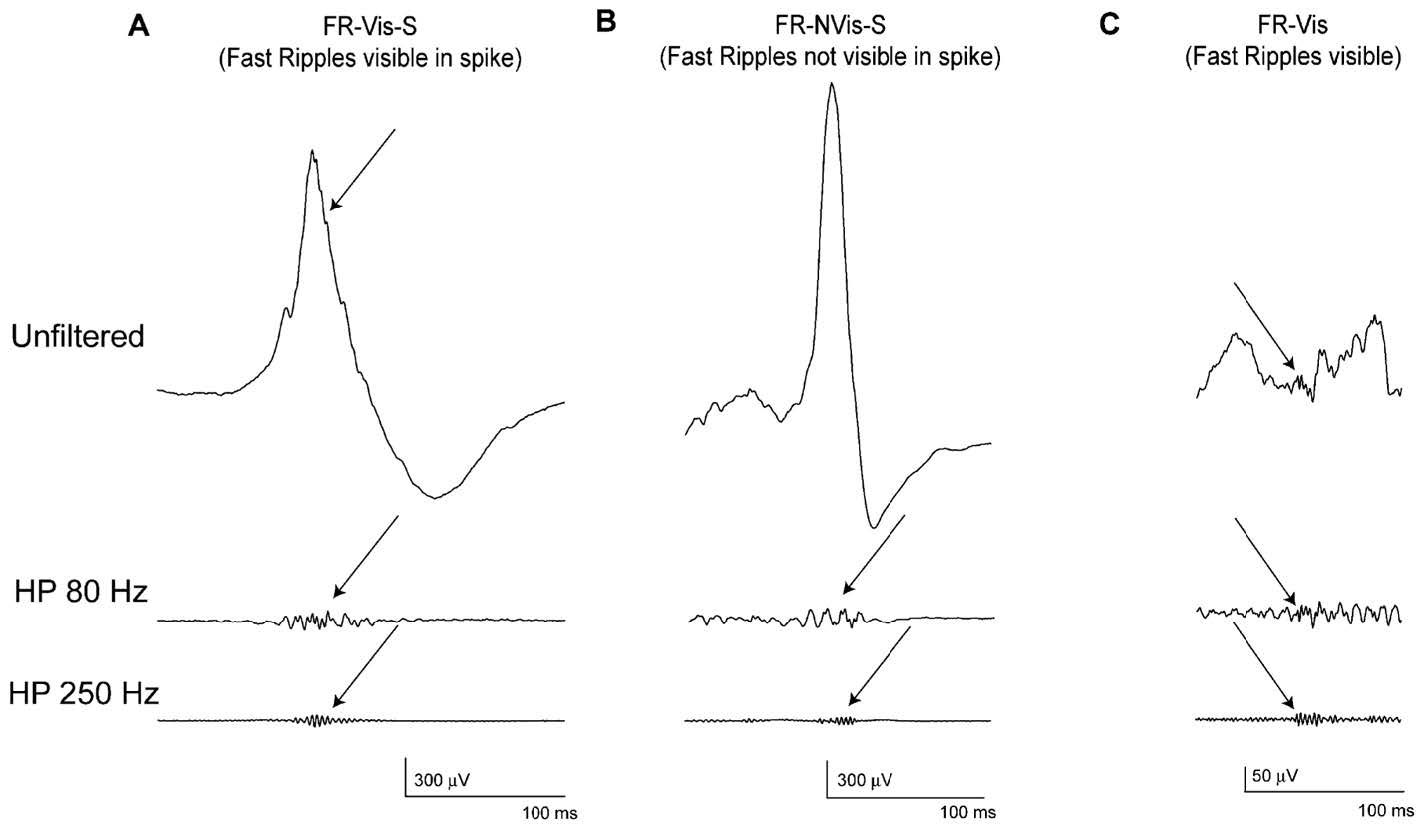
\includegraphics[width=1\textwidth]{Images/HFOsWithSpike.jpg}
\caption{HFO classification. (A) HFO visible in spike; (B) HFO not visible in spike; (C) HFO visible, independently of a spike. Top: non-filtered spike; middle: signal filtered with high-pass filter of 80Hz; bottom: signal filtered with high-pass filter of 250Hz. Image adapted from \citep{Urrestarazu2007}}
\label{fig:HfoSpike}
\end{figure}      

Due to the low signal-to-noise ratio of noninvasive electromagnetic signals at high frequencies \citep{Muthukumaraswamy2013}, HFOs are commonly detected in intracranial recordings. Visual marking of HFOs is highly time-consuming, but several automatic algorithms have been proposed both in the time and in the time-frequency domains \citep{Liu2016,Burnos2014,vonEllenrieder2012,Zelmann2012}. Time-frequency detectors are useful to reduce false positives because they exploit the assumption that an HFO should be a short-lived event with an isolated spectral peak at a distinct frequency \citep{Cho2012,Crepon2010}. 

The detection of HFOs in noninvasive signals is a field of increasing interest. Some recent studies have shown that HFOs can be detected in EEG \citep{Papadelis2016,Andrade-Valenca2011,Kobayashi2010,Zelmann2014} and in MEG \citep{vanKlink2015,vonEllenrieder2016,Nissen2016}. However, due to the high number of channels, the low signal-to-noise ratio of noninvasive techniques, and the lack of a well-established definition of HFOs, the automatic detection of these oscillations and the determination of the area generating them is still a challenging task. The noninvasive detection and localization of HFOs with MEG would significantly expand the clinical utility of these biomarkers that, to date, are only detected with patients with implanted intracranial electrodes.  

\subsection{Methods for noninvasive localization of the epileptic focus in MEG}

In the so-called inverse problem, source reconstruction methods are used to estimate where the activity recorded from the scalp was originated. Before such an estimate can be computed, a set of \emph{a priori} assumptions have to be computed to solve the forward problem, in which the scalp potentials and external fields for a specific set of neural current sources are computed \citep{Baillet2001}. 

The estimation of the induced magnetic fields is given by a \emph{Head Model}. The most common models used in most clinical and research applications are two: the \emph{spherical head models}, were the geometry of the head is fitted into spheres and the \emph{realistic head models}, that use the anatomical information obtained by MRI images. Two popular \textit{spherical head models} are the single sphere model \citep{Cuffin1977} that consist of a set of nested concentric homogeneous spherical shells representing brain, skull, and scalp \citep{Mosher1999,Zhang1995};  and the overlapping spheres model \citep{Huang1999}, where a sphere is fit separately for each sensor according to a local region of the surface closest to that sensor. To compute the volume conductor using a \textit{realistic head model},  two approaches can be used: the boundary element method (BEM) assumes isotropic and homogeneous tissues (brain, skull, scalp) obtaining simplified field equations that only depend on the surface (or boundary) of the  or the compartments \citep{Nolte2003}; and the finite element method (FEM) \citep{Ermer2001}, where the solution of the forward problem is solved for arbitrary, neither homogeneous nor isotropic, distributions resulting in equations that depend on the whole volume of the tissues. In order to solve the problem, the volume is divided into smaller pieces where an approximation of the solution is obtained. MEG measurements are less sensitive to the effects of volume currents than EEG, consequently, the simpler spherical head models work well for MEG but in the case of EEG, realistic head models have to be considered \citep{Baillet2001}.

\begin{figure}[ht]
\centering
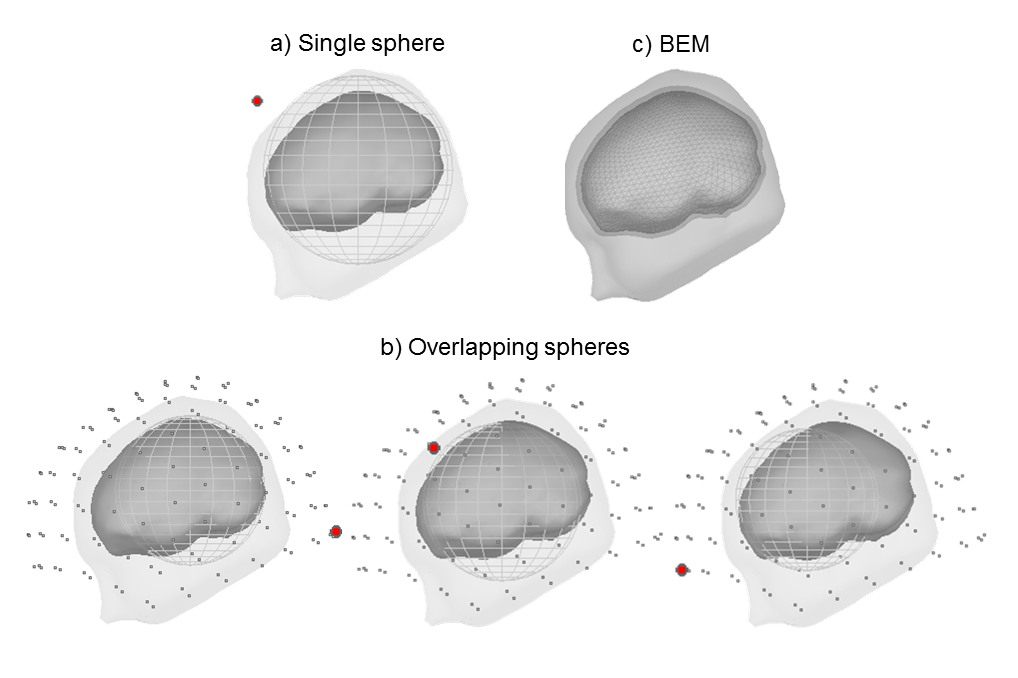
\includegraphics[width=1\textwidth]{Images/bemspheres.png}
\caption{Example of computation of a head model with a) a single sphere, b) with overlapping spheres (one sphere is computed for each channel) and c) BEM method. Head shapes and images generated with Brainstorm \citep{Tadel2011}}
\label{fig:headmodels}
\end{figure}      

Regarding MEG source estimation, several methods are available for that purpose: Equivalent current dipole (ECD), linear constrained minimum variance beamformer (LCMV-Beamfomer), synthetic aperture magnetometry (SAM), dynamic imaging of coherent sources (DICS), partial cannonical correlation/coherence (PCC), minimum norm estimation (MNE),  multiple signal classification (MUSIC), and low-resolution electromagnetic tomography (LORETA), among others. The following paragraphs focus on the first two: ECD and the LCMV-Beamformer techniques. ECD is commonly used to estimate the sources generating IEDs \citep{Stefan2003,Fischer2005,Oishi2006}; LCMV-Beamformer is a novel approach that, due to its performance as a spatial noise filter, has proven to be useful in reducing the high-frequency noise and to detect HFOs that were not visible at the scalp level \citep{vanKlink2015,Nissen2016}.  

\subsubsection{Equivalent current dipole}

Once the forward problem is solved, that is, the estimation of how the sources distribute through the volume is available, the ECD method uses this information and the data from scalp sensors to evaluate a set of parameter values that minimizes the difference between observations and predictions from the model. The minimization procedure is an iterative optimization problem that requires the specification of an initial guess of what the solution may be, that means, to specify the initial position and the number of dipoles. The risk of overfitting the data increases when the number of parameters with respect to the number of channels also increase \citep{Heller2014}. For this reason, no more than a few number of dipoles are set. To avoid local minima, the localization procedure is typically repeated several number of times using different starting points and selecting the solution that gives the best fit in each case.  

\begin{figure}[ht]
\centering
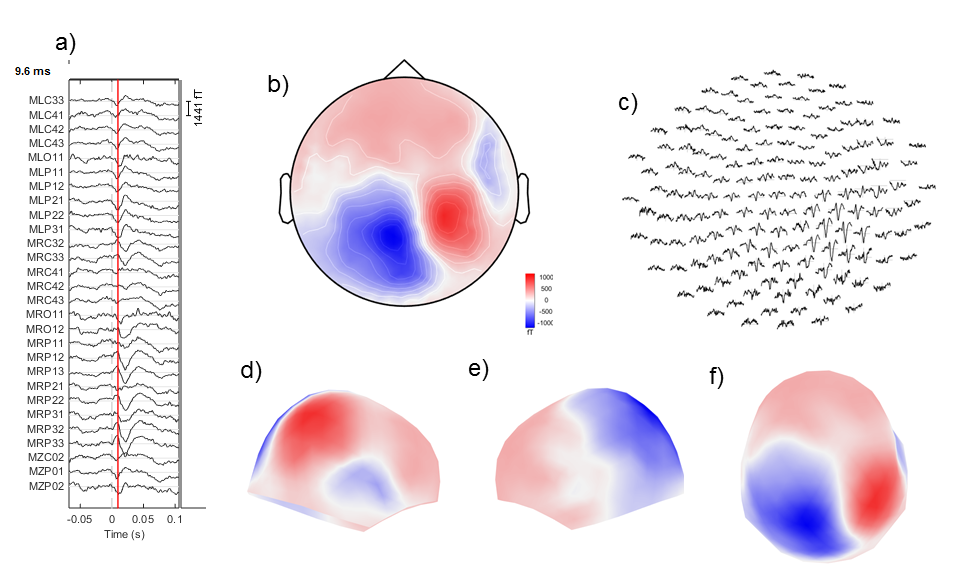
\includegraphics[width=1\textwidth]{Images/dipoles.png}
\caption{Visualization of a dipolar distribution in a) Most relevant scalp signals, b) Topographic disc c) Whole-sensor 2D image d), e) and f) 3D helmet activation map. Images generated with Brainstorm \citep{Tadel2011}}
\label{fig:dipolar}
\end{figure}   

Whenever it is reasonable to assume that an electromagnetic potential arises from a single or a few sources, dipole source localization is the simplest method to determine the center of the sources \citep{Lutkenhoner1998}. The dipolar nature of the electromagnetic signals was first observed in the fields obtained by evoked somatosensory responses \citep{Barnard1967}. The common practice to obtain the ECD from MEG data is to observe the scalp signals using different visualization approaches (see Figure \ref{fig:dipolar}) and look for dipolar patterns in the signals, such as the ones produced by IEDs. To evaluate the performance of the fitting algorithm, the \emph{goodness of fit} can be computed as the difference between the original scalp signals and the ones computed by the ECD model. The \emph{confidence volume} measure the intervals where the solution is plausible \citep{Heller2014}. The most common approach is to employ a Monte-Carlo technique generating a dipolar model with added noise and compute the ECD several times to see how the obtained dipole spread throughout the volume. In order to validate a dipole, high \emph{goodness of fit} values with low \emph{confidence volume} are expected. 

\subsubsection{Beamforming}
\label{sec:Bfanalysis}
Beamforming techniques were first developed for radar applications to amplify the sensitivity of specific sources of interest and to attenuate signals coming from other locations \citep{vanVeen1988}. This concept can be exploited using MEG and EEG signals under the main assumption that two distinct cortical areas are not linearly correlated in their activation \citep{vanVeen1997}. If signals are correlated, the beamforming analysis will return low power sources. 

Beamforming is a scanning technique that address the activation of a desired number of dipoles inside the head. The position and the number of the sources can be decided \textit{a priori}.  The purpose of this technique is to enhance the signals coming from a particular position, while reducing the signals coming from other directions \citep{Zhang2015}.  For this reason, is considered as an spatial filtering technique that passes the activity at the target location with unit gain while suppressing the contribution of other sources \citep{vanVeen1997}. 

\begin{figure}[ht]
\centering
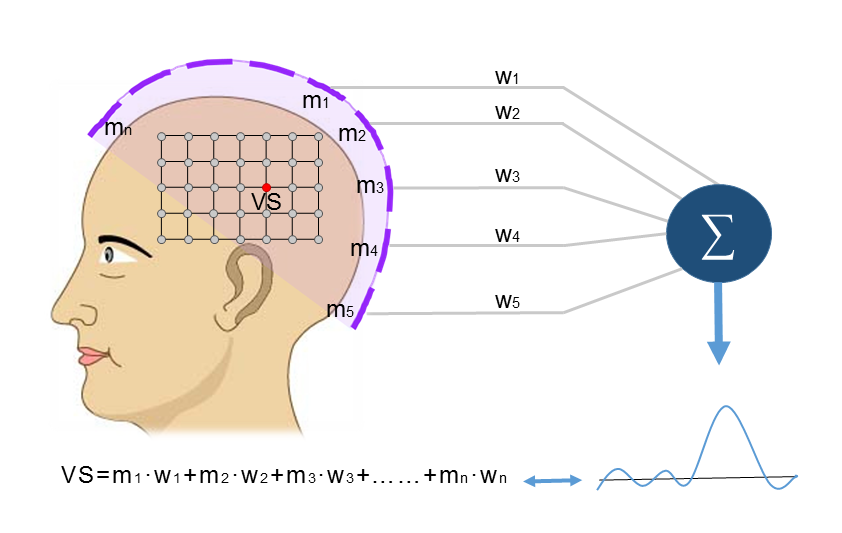
\includegraphics[width=1\textwidth]{Images/beamformer.png}
\caption{Schematic representation of beamforming analysis. The neuronal signal at a location of interest is estimated as the weighted sum of the MEG channels $(m_1...m_n)$ resulting into a Virtual Sensor (VS).}
\label{fig:beamformerVS}
\end{figure}   

The relationship between the scalp MEG signal $B$ and the neuronal sources is given by the following equation \citep{Hamalainen1993}:

\begin{equation}
B = LQ
\end{equation}

where the $(N \times 1)$ matrix $Q$ is the strength of the neuronal activity and $L$ is the leadfield matrix $(M \times N)$, with \emph{M} sensors and \emph{N} number of elements in the pre-defined source space. The leadfield is completely defined by the sensor configuration, the head model and the source model. The simplest source is the ECD explained in the previous section. 

With the observations from the scalp signals in time, $B(t)$, the strength for each neuronal source can be expressed as:
\begin{equation}
\label{eq:BF2}
	Q =C_{j} L^T C_b^{-1} B
\end{equation}
where $C_j$ and $C_b$ are the source current and data covariance matrices. The differences among Beamforming and other source reconstruction techniques rely on the assumption that is made about the source current covariance matrix \citep{Hillebrand2005}. Beamforming assumes that all sources are uncorrelated, i.e., $C_j$ is a diagonal matrix where each diagonal element, corresponding to a location $\theta$, can be related to the measured data as follows \citep{Mosher2003}:
\begin{equation}
\label{eq:BF3}
	\sigma_{\theta} =(L_{\theta}^T C_b^{-1} L_{\theta})^{-1}
\end{equation}
Combining equations \ref{eq:BF2} and \ref{eq:BF3} gives:
\begin{equation}
\label{eq:BF4}
	Q_{\theta}=(L_{\theta}^T C_b^{-1} L_{\theta})^{-1} L_{\theta}^T C_b^{-1} B = W_{\theta}^T B
\end{equation}
The value of the diagonal element  $C_j$  (Equation \ref{eq:BF3}) determines the eventual power of any source at a certain location $\theta$. If all the data covariance $C_{b}$ correspond to a single source, a maximum will be obtained in equation \ref{eq:BF3} but if this source shares variance with another, the estimated power $Q_{\theta}$ will decline. The effect of correlated activity depends on the distance between sources: for high correlated activity between two closely spaced sources the reconstruction might be erroneous and if the sources are well-separated those can be completely canceled \citep{vanVeen1997}. Still, beamforming have proven to be robust when dealing to partially correlated sources.

The Beamforming can be computed by dividing the source space into a tridimensional grid (or voxel space). In order to avoid false detection caused  by noise, the resulting 3D image must be normalized with respect to an estimation of the noise power \citep{Hillebrand2005,vanVeen1997}.  

Once the normalization is applied, the peaks of the beamforming 3D image can be obtained. An estimate of the time course of the neuronal activation of interest (or any point of the grid) can be achieved (see Figure \ref{fig:beamformerVS}). The positions where the time course of the neuronal sources are computed are commonly known as \emph{Virtual Sensors} (VS). Each virtual sensor time course signal is obtained as the weighted sum of each of the MEG sensor data, suppressing the signal from noise.  In section \ref{sec:BfSpatialFilter} the ability of LCMV-Beamformer to act as a spatial filter will be explained. 

\section{Artifacts and rejection techniques in MEG}

Brain signal recordings can be easily contaminated both by external noises and by interferences coming from inside the body, such as muscular or cardiac activities. The reduction of artifacts is a crucial step in signal analysis because meaningful physiological data can stay masked behind the artifactual activity, or even leading to inaccurate or wrong interpretation of the source of the signals. Thus, signal pre-processing is an imperative step to successfully localize epileptic focal activity. Many acquisition systems are able to reduce some artifacts related with external magnetic noise, stimulation, etc. However, there are other sources of artifacts present in the electromagnetic signals that cannot be reduced \emph{a priori}. In the following section, the most frequent artifacts in MEG data are described, as well as the most important techniques for its reduction. 

    \subsection{Physiological artifacts}
    
Physiological artifacts are generated by the patient itself and include cardiac, muscular, ocular, respiratory activity among many others. In this section, a brief description of the most common physiological artifacts is given, with special attention to muscular artifacts, which overlap the HFOs frequency band.

\textbf{Ocular artifact}
\\
The eye can be represented as a small electrical dipole oriented from the negatively charged retina to the positively charged cornea \citep{Croft2000}. When the eye moves, the orientation of the dipole changes, altering the associated electromagnetic fields in the frontal region, near the eyes. For example, blinks also generate artifacts due to the change in the intensity of the dipole created by the movement of the eyelid over the eyeball \citep{Hamalainen2004}.

\textbf{Cardiac artifact}
\\
The magnetic field of the heart is significantly larger than the normal or pathological brain activity. Its amplitude reaches a few hundred pT over the chest (around 100 times the amplitude of an epileptic spike). The magnitude of the cardiac artifact in MEG depends on the position of the head with respect to the heart \citep{Hamalainen2004}, and varies from subject to subject. Furthermore, in children recordings this interference may be stronger due to the shorter heart-to-brain distance.

\textbf{Muscular artifact}
\\
The power spectrum of a contracting muscle typically shows a bandwidth activity between 20 Hz to 300 Hz \citep{Criswell2011}. While most muscles near the jaw have peak frequencies around 20 Hz to 80 Hz, posterior head muscles (sternocleidomastoid, splenius capitis and trapezius) have higher peak frequencies (around 100 Hz) \citep{Muthukumaraswamy2013}. Studies in EEG blocking the neuromuscular activity with \textit{cistaracurium} \citep{whitham2007,whitham2008} showed that even in the electrodes in the center of the head the muscular activity produced a frequency spectrum around 10 times higher in the 80 Hz band. In MEG, there are currently no studies evaluating this effect, but is expected less muscular artifact since the magnetic fields falls off rapidly as distance increases to the primary dipole generators and secondary volume currents contribute little to the external MEG field\citep{Hamalainen1993}. This effect has been described in simultaneous MEG/EEG recordings \citep{Claus2012}. The main difference between muscular noise and high frequency oscillations is that the latter exhibit a more sinusoidal behaviour (grouped in a narrow frequency range) than former, which have a more spiky nature (contribution of a wider frequency range)
  

\subsection{Non-physiological artifacts}

The recordings can be contaminated by numerous non-physiological artifacts generated from the immediate subject surroundings. Common non-physiological artifacts include those generated by monitoring and electrical devices, and the power line (50 Hz or 60 Hz). In MEG recordings, most of these interferences are properly attenuated thanks to the Magnetically shielded room. Furthermore, MEG systems are highly sensitive to metallic interference. If the patient possess non-removable metallic devices, they considerably affect the recorded signal as the source of interference is inside the shielded room. 
 
\textbf{Metallic interference}
\\
MEG systems are sensitive to metallic ferromagnetic materials. Metallic interference may come from inside the head, such as implanted intracranial electrodes, dental ferromagnetic prosthesis or brackets, or from outside, such as pacemakers and vagal stimulators \citep{Vrba2002}. To try to minimize the effect of these interferences, an extremely magnetic hygiene inside the shielded room is required \citep{Hillebrand2013}. Recordings have to be performed with subjects trying to avoid any kind of movement, and even a demagnetization of the subject can be carried out. For this reason, MEG signal recording requires very careful preparation that can only be performed by highly trained specialists. Despite all precautions, sometimes it is not possible to eliminate all sources of metallic artifacts and highly distorted recordings are obtained. 

Typically, these artifacts appear modulated by breathing and cardiac rhythms \citep{Hillebrand2013} due to the great sensitivity to movement. The amplitude of metallic artifacts is typically much higher than the amplitude of cerebral signals and can even reach values larger than 100 fT \citep{Cheyne2007}. Metallic artifacts affect the whole record, overlapping brain activity, and may alter all head channels with varying amplitudes. Usually, there are a certain number of channels whose high level of contamination masks cerebral activity almost completely
        
    \subsection{Rejection techniques}
There are several useful methods to reduce interferences in electromagnetic multichannel signals. These can be simple methods such as band-pass or notch filtering to more advanced methods. In this section some of the most common and efficient methods to reduce MEG artifacts will be explained.   

    	\subsubsection{Blind source separation methods}

Blind source separation (BSS) can be used to decompose complex EEG or MEG data into simpler components based on statistical assumptions without using a physical forward model. The term \emph{source} here refers to an original signal while \emph{blind} indicates that no information is known about the mixing process of the sources \citep{Hyvarinen2001}. 
The first assumption that is made in BSS methods is that the recorded signals in the scalp are a mixture of the original signals (source). This problem can be mathematically described as: 
\begin{equation}
  x =As
\end{equation}

where $x$ is the recorded signal with $n$ channels and $s$ is the original signal with $m$ components. $A$ is the $n \times m$ mixing matrix. The second assumption is that the mixture is linear and the third is that some type of independence should exist between the original components. 

The BSS algorithms that exist differ on the statistical independence that is assumed. In general, the classification is divided into two main groups: the algorithms that use second order statistics (SOS) and those that exploit the high-order statistics of the signals (HOS).

The SOS methods only consider the correlation information to evaluate the independence between sources. The assumption implies that the components have no spatiotemporal or spatial time-frequency correlations between them \citep{James2005}. The mixing matrix is obtained taking into account a set of lagged covariances \citep{Hyvarinen2001}. One example of this kind of algorithms is the Algorithm for Multiple Unknown Signal Extraction (AMUSE), in which only two lags are considered \citep{Tong1991}. First of all, AMUSE decorrelates the signals at $\tau_0=0$, or in other words, applies a PCA to the input data. Secondly, the signals are decorrelated again but adding a time delay $\tau_1$ (usually equal to 1 sample). The main advantage of AMUSE lies on its low computational complexity \citep{Cichocki2005}. Although simple, SOS algorithms can deal with gaussian sources and are robust in presence of white noise \citep{James2005}.

The algorithms that employ the HOS to solve the BSS problem are commonly known as Independent Component Analysis (ICA) techniques. The probability distribution of the sources must be non-gaussian in order to be considered independent \citep{Hyvarinen2001}. Two of the most popular approaches are FastICA and Infomax algorithms. FastICA \citep{Hyvarinen2000} is a fast, fixed-point iterative algorithm which searches projections that maximize the non-gaussianity of the components by computing their kurtosis. Infomax relies on the information maximization principle \citep{Bell1995}. This algorithm maximizes the output entropy of a neural network with nonlinear outputs. The original Infomax is able to deal only with super-gaussian sources, however, the extended Infomax \citep{Lee1999} is able to estimate sub-gaussian sources. 

The performance of SOS and HOS algorithms in reducing artifacts from MEG and EEG signals has been tested in several studies \citep{Fatima2013,Breuer2014,Mantini2008,Escudero2011,Romero2008,Romero2009}. The algorithms listed above have shown different performances depending on the application or on the type of artifacts. For this reason, all of them are still used in the current applications, practice and research. 

\subsubsection{Signal space separation methods}

Signal space separation (SSS) is a method which takes into account the Maxwell equations for electromagnetism and is able to separate magnetic sources inside and outside the brain \citep{Taulu2004}. One of its main limitations is that artifacts from sources near the sensor array, such as metallic or dental implants, project into both subspaces and are not properly removed. For this reason, the method has been extended and termed as temporal Signal Space Separation (tSSS) \citep{Taulu2006}. These techniques have proven to be effective metallic interference \citep{Hillebrand2013}. However, they are only applicable to Elekta-Neuromag systems and their algorithms are not published and not freely available. 
        
        \subsubsection{Beamformer spatial filtering}
		\label{sec:BfSpatialFilter}

The beamformer algorithm act as a filter for activity in a target location of interest. This is known as \emph{spatial filtering} (Figure \ref{fig:spatialFilter}). The beamformer weights explained in the \ref{sec:Bfanalysis} section determine the spatial filtering characteristics of beamformer increasing the sensitivity in a region of interest and therefore attenuating the noise as well as the activity from other (remote) active brain regions \citep{Mosher2003}. While temporal filtering involves operating on times samples of a signal; spatial filtering involves processing spatial samples of a signal. The pass-band of the signal at the location of interest $\theta$ must have an unit response: 

\begin{equation}
\label{eq:sf1}
W_{\theta}^T B(\theta) = 1
\end{equation}
while at any other point $s$ must be satisfied:

\begin{equation}
W_{\theta}^T B(s) = 0
\end{equation}

In practice, to fully suppress the contribution of other sources is not possible. The idea behind LCMV-Beamformer\citep{vanVeen1997} used to address this problem is to find a $W_{\theta}^T$ minimize the signal power (or variance) maintaining the linear response constraint from equation \ref{eq:sf1}.

\begin{figure}
\centering
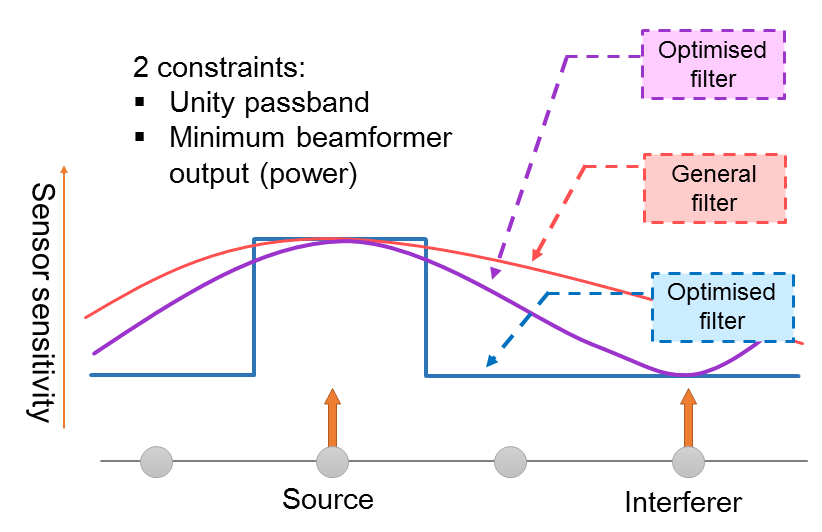
\includegraphics[width=0.8\textwidth]{Images/spatialfilter.png}
\caption{General scheme of the idea behind spatial filtering. The ideal spatial filtering is only sensitive to the source of interest and non-sensitive to other interference sources. In reality, it exists some spatial leakage. A general filter, such as dipole fitting procedure, do not actively suppress the interfering source. The LCMV-Beamforming is an optimized spatial filter that is not only sensitive to the source of interest but is also actively suppressing the interfering sources.}
\label{fig:spatialFilter}
\end{figure}      

The signal at each location in the brain is composed by three component dipole (each one oriented in a direction). Hence, three spatial filters for each location are computed. Each virtual sensor will have weighed contribution of the MEG sensors (see Figure \ref{fig:beamformerVS}) for each one of the locations. However, The interpretation of the source signals is facilitated if the posterior measurements are performed in if plain channels rather than a triplet of channels. The most common option is to project the time-series along the dipole direction that explains most variance. This projection is equivalent to determining the largest (temporal) eigenvector and can be computationally performed using the singular value decomposition (svd).


